\chapter{Incidencias}

\section{Visión general}

Durante el desarrollo del proyecto han surgido diversas incidencias que han ralentizado el desarrollo de este. A continuación se van a explicar algunas de las más importantes, así como la decisión que se ha tomado en cada una de ellas.

\section{Instalación Graph models}

La instalación de la extensión de Django en OS X 10.9.8, Graph models ha sido larga y ardua. Para hacer uso de esta herramienta se ha tenido que instalar primeramente django-extensions, el cual no supuso ningún problema, dado que era una dependencia de \acrshort{labman} y se descargó e instaló durante el proceso de instalación de \acrshort{labman}. Creyendo que simplemente con instalar django-extensions era suficiente para la generación de los modelos se procedió a la ejecución de un comando de consola de ejemplo que venía con la instalación de \acrshort{labman}.

Al ejecutarlo se produjo un error informando que las herramientas pygraph o pydot no estaban instaladas, por lo que se procedió a instalar pygraph por medio gestor de paquetes de Python pip\cite{pip} a través del comando \textit{pip install pygraph} o bien \textit{easy\_install pygraph}, sin embargo o bien no lo encontraba o daba un error por faltar la dependencia graphviz.

Se intentó descargar la dependencia en primera instancia por medio de pip o easy\_install, aunque pudo no encontrar ningún paquete con dicho nombre. Como segundo intento se procedió buscar la dependencia por Homebrew\cite{Homebrew}, sin éxito alguno.

Se procedió como último intento a buscar en el repositorio web de MacPorts\cite{MacPorts} la existencia de graphviz y pygraph. Al verificar la existencia de estos paquetes en su repositorio, comenzó el proceso de descargar el paquete de instalación necesario para instalar MacPorts. Una vez instalado se introdujeron los comandos de instalación de ambos paquetes produciendose un error con el rsync. Al parecer, la Universidad de Deusto tiene algún puerto necesario para conectarse al repositorio cerrado por lo que se tuvo que crear un punto \acrshort{wifi} desde un dispositivo móvil conectado a una red privada \acrshort{3g} para descargar los paquete.

Al comenzar el proceso de instalación saltó una alerta sobre la ausencia de la herramienta de desarrollo Xcode\cite{Xcode} por lo que no se podrían compilar los paquetes. Se tuvieron que eliminar los archivos temporales que había generado MacPorts, descargar Xcode y aceptar la licencia de uso para finalmente poder instalar graphviz, lo que permitiría instalar por fin las dependencias pygraph y pydot para la ejecución del comando Graph models y generar los grafos adjuntados en esta memoria en el capítulo \ref{chap:design}.

\section{Despliegue del servidor OAI-PMH en Apache}

Antes del despliegue final en producción del servidor \acrshort{oaipmh} en el servidor \acrshort{http} Unicorn\cite{Unicorn}, se ha realizado un despliegue en un servidor Apache público para poder realizar pruebas con clientes \acrshort{oaipmh} web. No ocurrió ningún incidente durante el proceso de instalación de Apache en OS X, sin embargo la configuración fue tediosa.

En primer lugar se tuvo que localizar los ficheros de configuración y \textit{logs} del servidor Apache para OS X, estos se encontraban \textit{/etc/apache2} y \textit{/var/log/apache2} respectivamente.

Como el servidor de \acrshort{oaipmh} es una aplicación basada en \acrfull{wsgi} se tenía que modificar el fichero \textit{httpd.conf} para que el servidor Apache cargase el módulo necesario para la ejecución de este tipo de aplicaciones. Se siguió el tutorial de configuración rápida para mod\_wsgi (Módulo \acrshort{wsgi}) en la \textit{wiki} de la página del proyecto en Google Code\cite{GoogleCode} para hacer una aplicación de prueba y comprobar que el módulo se había cargado correctamente\cite{WSGI_tutorial}.

Se procedió a crear un \textit{VirtualHost} para hacer referencia al servidor \acrshort{oaipmh} por medio de una \acrshort{url}, sin embargo no se consiguió configurar adecuadamente, al hacer una petición por medio de un navegador web no se recibía respuesta alguna y el \textit{log} de Apache no registraba ningún error en las peticiones, por lo que se abandonó la idea de configurar el \textit{Virtual Host}.

Se optó por una solución menos elegante, pero así mismo funcional, se configuraría el \textit{WSGIScriptAlias} para poder hacer referencia a la aplicación \acrshort{wsgi} por medio de la dirección \acrshort{ip} de la máquina que ejecutaría el servidor desde un cliente externo al local.

Se intento realizar una nueva petición desde el navegador y esta vez si se obtuvo respuesta. Si bien no era la respuesta que se deseaba, al ser un error interno el servidor, la información de la petición quedó registrado en los \textit{logs}, por lo que fue más sencillo hacer un seguimiento hasta el origen del mismo. Se descubrió que Apache no ejecutaba el entorno virtual con el que se aislaba la instalación de Python y sus dependencias. 

A lo largo del desarrollo del servidor se habían utilizado varias versiones de Python como la 2.5, 2.6 y 2.7, trabajando la versión final en la 2.6. Sin embargo, Apache estaba ejecutando los fragmentos residuales del código desactualizado de la versión 2.7. Se estudiaron las posibles soluciones al problema y se decidió actualizar el código de la versión 2.7 con aquel desarrollado en la versión 2.6 tras descubrir que no había incompatibilidades en el código.

Tras realizar este cambio, el servidor fue desplegado correctamente. Se hicieron pruebas con clientes externos a la máquina local para comprobar que realmente se podía acceder al servidor y se procedió a realizar un redireccionamiento de puertos en el Router para hacer el servidor \acrshort{oaipmh} público y realizar las últimas pruebas con clientes web que requerían la \acrshort{url} del servidor para descargar los datos y realizar las validaciones.

\section{Escapar caracteres especiales de JSON}

Gracias a las pruebas unitarias realizadas en el método \textit{oai\_query} que se tuvo que implementar en la capa de \acrshort{bd} del servidor MOAI se descubrió que varios de los campos recolectados podían contener caracteres de control como los que se muestran en la figura \ref{fig:json_string}.

\begin{figure}[!htbp]
	\centering
	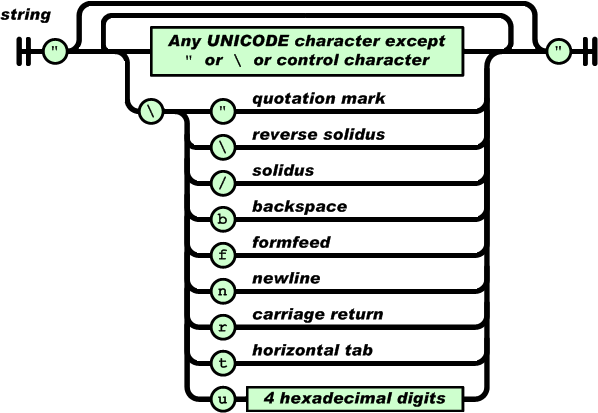
\includegraphics[scale=0.5]{fig/json_string}
	\caption{Definición de ``string'' de \acrshort{json}}
	\label{fig:json_string}
\end{figure}

Para evitar que surgieran errores se tuvo que implementar un método que eliminase estos caracteres te control o los escapase tal y como se muestra en el algoritmo \ref{lst:escaping_control_characters}

\lstinputlisting[language=Python, frame=single, label={lst:escaping_control_characters}, caption=Escapado o eliminación de caracteres de control de \acrshort{json}]{content/code/python/escaping_control_characters.py}
